\documentclass[11pt]{article}
\usepackage[margin=0.8in]{geometry}
\usepackage{amsmath,amssymb,booktabs,graphicx,longtable,array}
\usepackage[hidelinks]{hyperref}
\newcommand{\Sm}{\Sigma^{\mathrm m}}
\title{Direct finite-time entropy sampling for the three-mode NLS chain}
\author{Numerical audit report}
\date{1 September 2026}

\begin{document}
\maketitle

\section{Question and frozen calculation}

The calculation tests whether ordinary sampling resolves both signs of the
finite-time entropy observable for the smallest chain with an unforced middle
mode.  The parameters are
\[
n=3,\qquad T_L=10,\quad T_R=2,\quad \gamma=0.1,
\quad \Delta t=5\times10^{-4}.
\]
After burn-in time 500, the simulation records 7,813 non-overlapping blocks of
length 20 in each of 128 independent streams, giving 1,000,064 base blocks.
The accumulated observables are
\[
 \Sm=-\frac{Q_L}{T_L}-\frac{Q_R}{T_R},\qquad
 R_E=Q_L+Q_R-\Delta E,
\]
together with the middle-bond action current and the five-dimensional reduced
state at both block endpoints.  Longer horizons are formed only by grouping
consecutive blocks within the same stream.

The mean rates in the base data are
\[
 \langle Q_L/t\rangle=6.22090943,\quad
 \langle Q_R/t\rangle=-6.22091138,\quad
 \langle\Sm/t\rangle=2.48836475,
\]
and the mean action current is 1.25228320.  All eight batches completed, with
zero midpoint failures.

\section{Raw negative-tail resolution}

\begin{table}[ht]
\centering
\small
\begin{tabular}{rrrrrc}
\toprule
$t$ & blocks & $\#\{\Sm<0\}$ & $P(\Sm<0)$ & 95\% stream-bootstrap CI & paired bins \\
\midrule
20  & 1,000,064 & 41 & $4.09974\times10^{-5}$ & $[2.89981,5.39965]\times10^{-5}$ & 0 \\
40  & 499,968 & 0 & 0 & $[0,0]$ & 0 \\
60  & 333,312 & 0 & 0 & $[0,0]$ & 0 \\
80  & 249,984 & 0 & 0 & $[0,0]$ & 0 \\
100 & 199,936 & 0 & 0 & $[0,0]$ & 0 \\
120 & 166,656 & 0 & 0 & $[0,0]$ & 0 \\
140 & 142,848 & 0 & 0 & $[0,0]$ & 0 \\
160 & 124,928 & 0 & 0 & $[0,0]$ & 0 \\
180 & 111,104 & 0 & 0 & $[0,0]$ & 0 \\
200 & 99,968 & 0 & 0 & $[0,0]$ & 0 \\
\bottomrule
\end{tabular}
\caption{Raw negative-medium-entropy counts. ``Paired bins'' is the number of
predeclared symmetric Freedman--Diaconis bin pairs having at least 20 raw
counts on each side.}
\end{table}

The predeclared direct-resolution gate requires at least 1,000 negative blocks
and at least eight symmetric bin pairs with 20 counts on both sides.  No
horizon passes.  Consequently no detailed-symmetry slope, confidence interval,
or $R^2$ can be estimated from these data without replacing raw tail counts by
an extrapolation.  No fit window was selected and no cloning run was
substituted.

\begin{figure}[ht]
\centering
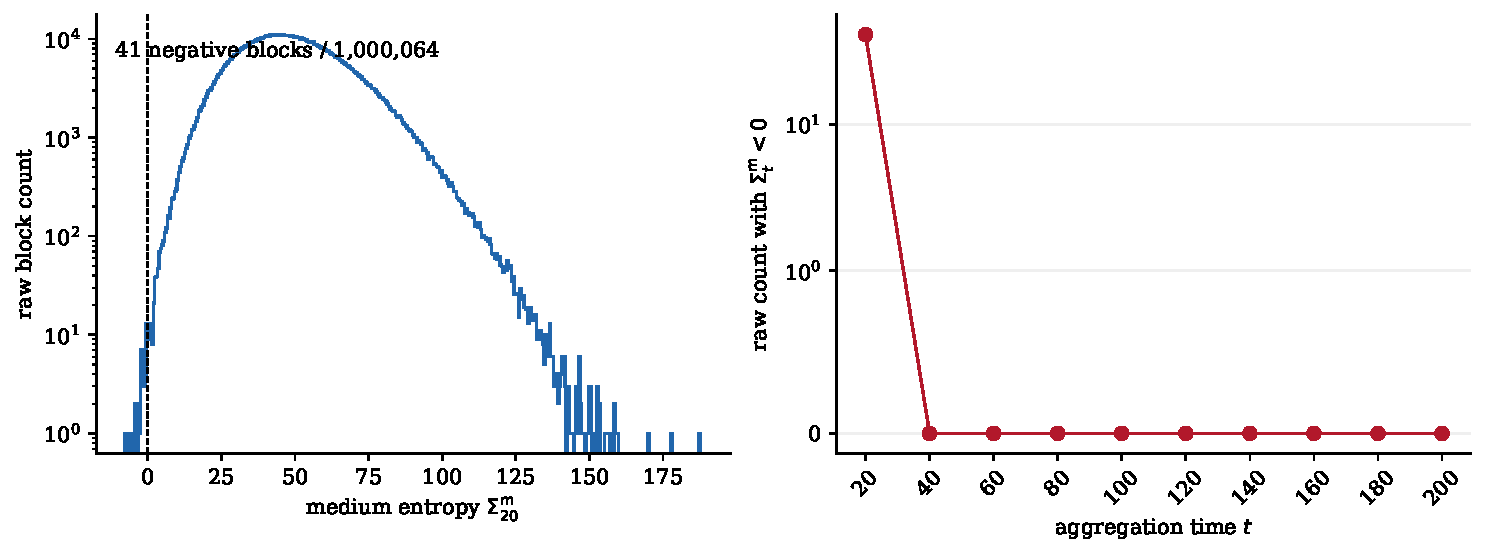
\includegraphics[width=0.96\textwidth]{figures/negative_tail_support.pdf}
\caption{Left: the raw $t=20$ medium-entropy histogram.  Right: negative-event
counts after within-stream aggregation.}
\end{figure}
\clearpage

\section{First-law residual}

\begingroup
\scriptsize
\setlength{\tabcolsep}{3pt}
\begin{longtable}{rrrrrrrrr}
\caption{Complete reported distribution summary of
$R_E=Q_L+Q_R-\Delta E$.}\label{tab:balance}\\
\toprule
$t$ & mean & std & RMS & min & 2.5\% & median & 97.5\% & max \\
\midrule
\endfirsthead
\toprule
$t$ & mean & std & RMS & min & 2.5\% & median & 97.5\% & max \\
\midrule
\endhead
20  & \texttt{-1.417e-5} & \texttt{2.970e-4} & \texttt{2.974e-4} & \texttt{-4.847e-3} & \texttt{-6.146e-4} & \texttt{-1.664e-5} & \texttt{6.077e-4} & \texttt{3.843e-3} \\
40  & \texttt{-2.834e-5} & \texttt{4.187e-4} & \texttt{4.196e-4} & \texttt{-4.997e-3} & \texttt{-8.644e-4} & \texttt{-3.272e-5} & \texttt{8.421e-4} & \texttt{3.994e-3} \\
60  & \texttt{-4.251e-5} & \texttt{5.124e-4} & \texttt{5.142e-4} & \texttt{-5.463e-3} & \texttt{-1.057e-3} & \texttt{-4.814e-5} & \texttt{1.011e-3} & \texttt{4.172e-3} \\
80  & \texttt{-5.668e-5} & \texttt{5.907e-4} & \texttt{5.934e-4} & \texttt{-5.268e-3} & \texttt{-1.229e-3} & \texttt{-6.281e-5} & \texttt{1.153e-3} & \texttt{4.313e-3} \\
100 & \texttt{-7.080e-5} & \texttt{6.612e-4} & \texttt{6.650e-4} & \texttt{-5.750e-3} & \texttt{-1.373e-3} & \texttt{-7.771e-5} & \texttt{1.276e-3} & \texttt{4.642e-3} \\
120 & \texttt{-8.502e-5} & \texttt{7.228e-4} & \texttt{7.278e-4} & \texttt{-5.629e-3} & \texttt{-1.508e-3} & \texttt{-9.181e-5} & \texttt{1.380e-3} & \texttt{4.520e-3} \\
140 & \texttt{-9.919e-5} & \texttt{7.825e-4} & \texttt{7.888e-4} & \texttt{-5.447e-3} & \texttt{-1.641e-3} & \texttt{-1.073e-4} & \texttt{1.481e-3} & \texttt{4.270e-3} \\
160 & \texttt{-1.133e-4} & \texttt{8.352e-4} & \texttt{8.428e-4} & \texttt{-5.493e-3} & \texttt{-1.759e-3} & \texttt{-1.204e-4} & \texttt{1.561e-3} & \texttt{4.755e-3} \\
180 & \texttt{-1.275e-4} & \texttt{8.856e-4} & \texttt{8.948e-4} & \texttt{-5.179e-3} & \texttt{-1.863e-3} & \texttt{-1.367e-4} & \texttt{1.657e-3} & \texttt{4.336e-3} \\
200 & \texttt{-1.416e-4} & \texttt{9.347e-4} & \texttt{9.454e-4} & \texttt{-5.267e-3} & \texttt{-1.972e-3} & \texttt{-1.478e-4} & \texttt{1.736e-3} & \texttt{4.418e-3} \\
\bottomrule
\end{longtable}
\endgroup

At $t=20$, the residual RMS is $2.97383\times10^{-4}$, or
$2.24426\times10^{-6}$ of the RMS left-bath heat.  Entropy and balance columns
recompute from the saved heat and energy fields within binary64/CSV roundoff;
all consecutive reduced endpoints agree exactly after parsing.
\clearpage

\section{Medium-only integral diagnostic}

\begin{table}[ht]
\centering
\small
\begin{tabular}{rrrrr}
\toprule
$t$ & $\log\langle e^{-\Sm}\rangle$ & 95\% CI & weight ESS & largest share \\
\midrule
20  & $-5.7736$ & $[-8.0682,-4.8381]$ & 2.288 & 0.6155 \\
40  & $-27.7021$ & $[-29.0827,-27.0673]$ & 4.967 & 0.3126 \\
60  & $-52.4555$ & $[-54.2741,-51.7400]$ & 3.780 & 0.3542 \\
80  & $-73.5308$ & $[-87.8362,-72.4322]$ & 1.000 & 1.0000 \\
100 & $-106.9585$ & $[-119.3689,-105.6540]$ & 1.169 & 0.9214 \\
120 & $-135.1248$ & $[-154.3239,-134.0262]$ & 1.000 & 1.0000 \\
140 & $-178.9688$ & $[-198.5417,-177.8702]$ & 1.000 & 1.0000 \\
160 & $-219.2272$ & $[-229.2468,-218.1317]$ & 1.030 & 0.9852 \\
180 & $-246.6478$ & $[-265.0109,-245.5492]$ & 1.000 & 0.9999 \\
200 & $-299.5255$ & $[-307.3934,-298.4274]$ & 1.188 & 0.9135 \\
\bottomrule
\end{tabular}
\caption{Medium-entropy-only exponential averages.  ESS and largest weight
share show that these averages are controlled by only one to five effective
samples and are not resolved rare-event estimators.}
\end{table}

These values are reported as requested but are not a total-entropy integral FT
test: the system-entropy endpoint contribution is omitted, and the exponential
average has extremely low tail ESS.

\begin{figure}[ht]
\centering
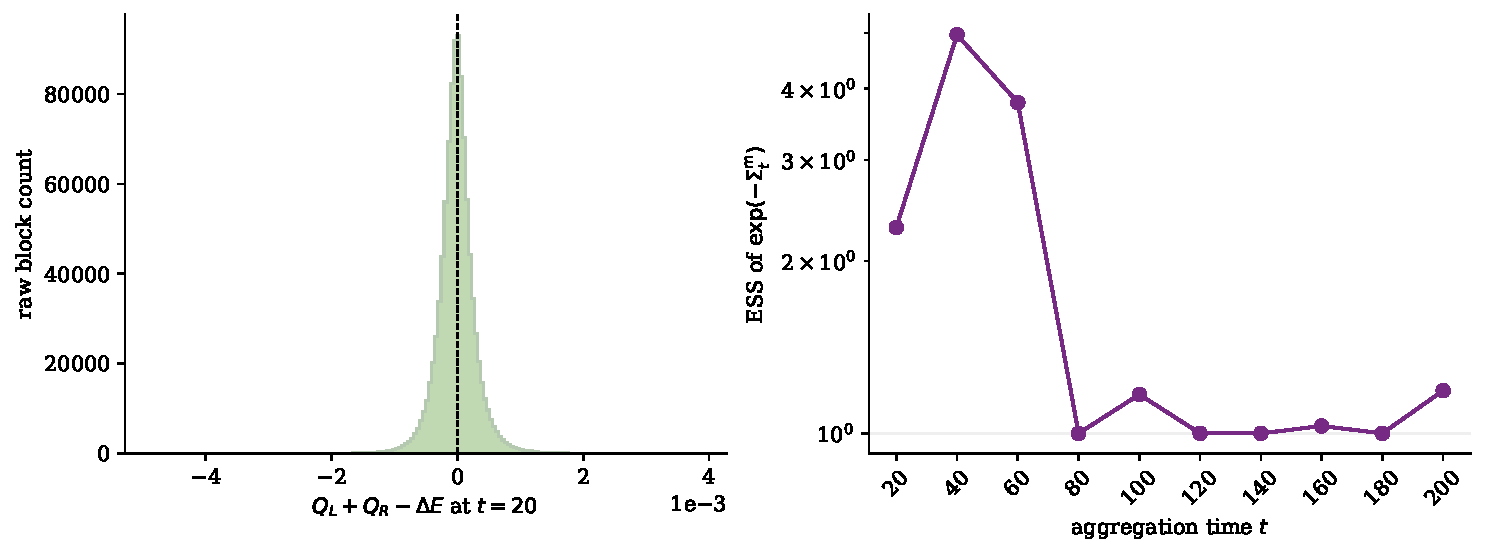
\includegraphics[width=0.96\textwidth]{figures/balance_and_ift_resolution.pdf}
\caption{Left: raw $t=20$ first-law residuals.  Right: effective sample size
of the medium-entropy exponential weights.}
\end{figure}
\clearpage

\section{Stationary-density limitation and provenance}

The saved Section-4 network
\texttt{KDE/4:15\_NN/h5\_files/final.keras} has SHA-256
\texttt{906f5e60...bc07d536}.  Its executed notebook uses
$(T_1,T_3)=(2,8)$, not $(10,2)$.  It also reports scaled log-density RMSE
0.409876 and mean normalized Fokker--Planck residual 0.3733.  Applying that
network to these endpoints would not provide the requested stationary density.
Therefore $\Delta s_{\rm sys}$, the total-entropy detailed slope, and the
total-entropy integral FT are not evaluated.

The production executable used Git commit
\texttt{9fd7d75a45a45473a82a380e615f7b97c4a4176c}, source SHA-256
\texttt{9ae5835e...6d4eaf2}, binary SHA-256
\texttt{15436d39...7be18e}, and seed 2026083133.  The raw block file has
SHA-256 \texttt{4f728b3d...7d7a088f}.  The exact command and complete hashes
are recorded in \texttt{provenance/production\_manifest.txt}.

\section{Strict outcome}

Direct sampling at $n=3$ does not resolve the negative tail sufficiently for a
detailed finite-time FT fit: only 41 negative blocks occur at $t=20$, and none
occur at $t\ge40$.  This is a support limitation, not evidence for or against
the fluctuation theorem.  Cloning or another rare-event method may now be
considered, but none was started as part of this direct-sampling experiment.

\end{document}
